\documentclass[conference,10pt,letterpaper]{IEEEtran}

\usepackage{amsmath,amssymb,amsfonts}
\usepackage{array}
\usepackage{booktabs}
\usepackage{cite}
\usepackage{graphicx}
\usepackage{float}
\usepackage[expansion=false]{microtype}
\usepackage{textcomp}
\usepackage{url}
\usepackage{hyperref}

\graphicspath{{./}{figures/}}

\makeatletter
\@ifclassloaded{IEEEtran}{}{%
  \usepackage[margin=1.75cm]{geometry}
  \providecommand{\IEEEauthorblockN}[1]{#1}
  \providecommand{\IEEEauthorblockA}[1]{\textit{#1}}
  \providecommand{\IEEEPARstart}[2]{\textbf{#1}#2}
  \newenvironment{IEEEkeywords}{\vspace{4pt}\noindent\textbf{\textit{Keywords---}}\ignorespaces}{\par\vspace{6pt}}
}
\makeatother

\hypersetup{colorlinks=true, linkcolor=black, citecolor=black, urlcolor=blue}

\begin{document}

\title{CaneSugar Neural v1: A Deep Tabular Highway Network for Sugarcane Yield Prediction}

\author{
\IEEEauthorblockN{Haarini S}
\IEEEauthorblockA{
CSE Department\\
Kongu Engineering College\\
haarinis.23cse@kongu.edu
}
\and
\IEEEauthorblockN{Gowtham C D}
\IEEEauthorblockA{
CSE Department\\
Kongu Engineering College\\
gowthamcd.23cse@kongu.edu
}
\and
\IEEEauthorblockN{Harini Priya M}
\IEEEauthorblockA{
CSE Department\\
Kongu Engineering College\\
harinipriyam.23cse@kongu.edu
}
}

\maketitle

%====================================================================
\begin{abstract}
Sugarcane yield forecasting across commercial smallholder tracts is complicated by long vegetative cycles (10--18 months) and non-linear interactions among soil chemistry, fertilizer schedules, and seasonal moisture deficits. While gradient-boosted decision trees remain the operational benchmark for tabular crop data, their orthogonal step functions produce discontinuous response surfaces that cannot model continuous physiological responses or provide calibrated prediction intervals. Conversely, standard feedforward networks frequently underperform on agricultural tables due to gradient dispersion across deep bottlenecks and high-dimensional sparsity from one-hot categorical encodings.

To address these limitations, we designed \textbf{CaneSugar Neural v1}, a domain-tailored deep tabular architecture for plot-level yield prediction. The model combines 20 categorical entity embeddings (100 total latent dimensions) with 65 continuous soil and climate measurements normalized via Layer Normalization, forming a unified 165-dimensional representation. A linear highway skip connection projects activations from the 128-unit intermediate layer directly into the 64-unit bottleneck, preserving early agronomic feature interactions during backpropagation. Training is regularized using Huber loss ($\delta = 1.0$) with decoupled weight decay under a cosine annealing schedule to limit the influence of severe weather outliers.

Evaluated on 450 held-out test plots from a 3,000-record field dataset partitioned 70/15/15, the standalone architecture achieves $R^2 = 0.9240$, a mean absolute error of 21.84~Q/A, root mean squared error of 29.72~Q/A, and mean absolute percentage error of 8.82\%. Across five independent runs with distinct random seeds, test performance remained consistent ($R^2 = 0.9247 \pm 0.0013$), outperforming CatBoost ($R^2 = 0.9081$), XGBoost ($0.8794$), and Random Forest ($0.8347$) baselines without ensembling. Epistemic uncertainty is estimated at inference through Monte-Carlo Dropout ($T = 30$ forward passes), yielding confidence intervals that widen under extreme inputs. Global attribution via Integrated Gradients identifies stalk volume (28.4\%), nitrogen application rate (14.2\%), and root-zone moisture (11.8\%) as the primary positive yield drivers.
\end{abstract}

\begin{IEEEkeywords}
Sugarcane yield prediction, deep tabular learning, entity embeddings, precision agriculture, Monte-Carlo Dropout, Integrated Gradients, residual highway networks.
\end{IEEEkeywords}

%====================================================================
\section{Introduction}

\IEEEPARstart{S}{ugarcane} (\textit{Saccharum officinarum} L.) accounts for roughly 80\% of worldwide sucrose production and serves as a primary feedstock for industrial bioethanol and co-generation grids~\cite{canata2024ai}. Because the crop requires an extended vegetative cycle spanning 10 to 18 months, yield forecasts generated mid-season directly dictate supply agreements, harvest scheduling, and mill crushing capacity~\cite{somard2024sugarcane}. For individual farm managers, accurate plot-level estimates provide actionable timing for nitrogen top-dressing and supplemental irrigation before the crop canopy closes.

\subsection{Agricultural Context}
Unlike annual cereal crops, sugarcane accumulates stalk tonnage and sucrose continuously across distinct tillering, grand growth, and ripening phases. In South Asian cultivation tracts, commercial harvest yield is universally recorded in Quintals per Acre ($1\text{ Q/A} = 100\text{ kg/acre} \approx 0.247\text{ t/ha}$). Final yield depends on the co-action of five distinct physical domains:
\begin{enumerate}
    \item Soil physicochemical baseline: root-zone depth, pH, electrical conductivity, Walkley-Black organic carbon, and sand--silt--clay textural distributions.
    \item Macronutrient and micronutrient availability: nitrogen, phosphorus, and potassium application rates alongside trace elements (Zn, Fe, Cu, Mn, B) that govern enzymatic tillering.
    \item Hydrological balance: cumulative seasonal rainfall, reference evapotranspiration ($ET_o$), shallow water table access, and irrigation method (drip versus furrow delivery).
    \item Thermal regimes: mean seasonal temperature, diurnal temperature fluctuations ($T_{\max} - T_{\min}$) driving sucrose accumulation, and total sunshine duration.
    \item Biometric stand architecture: millable stalk height, stalk diameter, tillers per linear metre, and planting density.
\end{enumerate}

\subsection{Problem Statement}
These variables interact through strongly non-linear biological thresholds. Nitrogen fertilization increases vegetative biomass following the law of diminishing returns, yet excessive application promotes crop lodging, suppresses sucrose content, and heightens vulnerability to red rot caused by \textit{Colletotrichum falcatum}~\cite{socadagui2026spatial}. Furthermore, according to Liebig's Law of the Minimum, crop response to nitrogen drops to zero if root-zone moisture or available potassium falls below critical survival thresholds~\cite{everingham2016accurate,inman2005sugarcane}.

Two computational paradigms historically dominate crop yield forecasting. Process-based biophysical simulation models, including DSSAT-CANEGRO~\cite{singels2005modelling} and APSIM-Sugarcane~\cite{keating1999modelling}, integrate differential equations governing carbon assimilation and transpiration. Although physiologically grounded, these systems demand exhaustive cultivar parameters and soil hydraulic calibration profiles rarely available for smallholder farms. 

Conversely, empirical tree ensembles such as Random Forest~\cite{breiman2001random}, XGBoost~\cite{chen2016xgboost}, and CatBoost~\cite{prokhorenkova2018catboost} serve as standard baselines for tabular datasets~\cite{van2020crop,silva2020sugarcane}. Nevertheless, decision trees partition feature space into orthogonal axis-aligned hyper-rectangles. This structure induces piecewise-constant step functions that misrepresent gradual crop responses to fertilizer or water gradients. Moreover, tree ensembles lack a unified mechanism to output calibrated Bayesian prediction intervals or generate exact input gradients for sensitivity analysis.

\subsection{Motivation and Contributions}
Multi-layer perceptrons often struggle against gradient-boosted trees on tabular benchmarks~\cite{shwartz2022tabular,borisov2022deep}. On agricultural records, this performance gap stems from two structural factors: one-hot encoding expands high-cardinality categorical variables into sparse vectors prone to overfitting, while stacking conventional dense layers causes gradient attenuation across deep bottlenecks, washing out subtle nutrient interaction ratios~\cite{gorishniy2021revisiting}.

To overcome these structural limitations, we developed CaneSugar Neural v1. This work offers five primary contributions:
\begin{enumerate}
    \item A specialized tabular architecture combining learned entity embeddings for 20 categorical variables with layer-normalized continuous features, merged into a unified 165-dimensional latent representation.
    \item A highway skip connection linking the 128-unit dense layer directly to the 64-unit bottleneck, providing a direct linear gradient path that preserves early nutrient-interaction signals during training.
    \item Robust optimization using Huber loss ($\delta = 1.0$) combined with decoupled AdamW weight decay and cosine annealing, preventing extreme field disruptions from distorting regression weights.
    \item Epistemic uncertainty quantification through Monte-Carlo Dropout ($T = 30$ passes), delivering per-plot confidence bounds that reflect out-of-distribution feature spaces.
    \item Transparent model attribution via Integrated Gradients, confirming that internal parameter sensitivities align with established agronomic response curves.
\end{enumerate}

\subsection{Research Questions}
This investigation evaluates six specific empirical questions:
\begin{itemize}
    \item \textbf{RQ1}: Can a standalone, non-ensemble deep neural network achieve $R^2 > 0.90$ on heterogeneous smallholder sugarcane field records?
    \item \textbf{RQ2}: Does domain-informed agronomic feature engineering (Liebig ratios, stalk geometry) provide measurable accuracy gains over raw field variables?
    \item \textbf{RQ3}: Do learned categorical embeddings improve generalization relative to traditional one-hot encodings?
    \item \textbf{RQ4}: Does the highway skip connection measurably stabilize gradient backpropagation and prevent validation loss degradation?
    \item \textbf{RQ5}: How sensitive is model convergence across multiple independent training runs initiated with distinct random seeds?
    \item \textbf{RQ6}: Do the most influential input features identified by Integrated Gradients match established physiological principles of cane growth?
\end{itemize}

%====================================================================
\section{Related Work}

\subsection{Sugarcane Yield Estimation}
Statistical yield forecasting historically relied on empirical regressions against seasonal climate indices. Everingham et al.~\cite{everingham2016accurate} demonstrated that Random Forests calibrated on regional Southern Oscillation and rainfall indices consistently outperformed traditional bivariate regressions across Australian sugarcane districts. Subsequent efforts incorporated multispectral remote sensing. Canata et al.~\cite{canata2024ai} related vegetation indices derived from orbital platforms to stalk Brix and juice purity, illustrating that spectral reflectance tracks sucrose maturity.

Recent investigations concentrate on sub-field spatial heterogeneity. Socadagui-Casas et al.~\cite{socadagui2026spatial} examined how soil compaction profiles and irrigation schedules co-vary to create sharp yield gradients within individual Colombian production blocks. Som-ard et al.~\cite{somard2024sugarcane} coupled unmanned aerial vehicle (UAV) imagery with Sentinel-2 time series across Thai plantations. While canopy reflectance correlated well with biomass during early dry phases, optical signals saturated once canopies closed and suffered data gaps during monsoon cloud cover. More critically, satellite radiometers record only surface canopy greenness; they cannot measure subsurface organic carbon, available potassium fractions, or root-zone moisture tension, which directly govern stalk elongation.

\subsection{Machine Learning in Crop Production}
In a systematic survey spanning over 500 agricultural studies, van Klompenburg et al.~\cite{van2020crop} identified Random Forest, support vector machines, and gradient boosting as the predominant algorithms for crop yield prediction. Silva et al.~\cite{silva2020sugarcane} evaluated XGBoost against feedforward neural networks on Brazilian mill datasets, finding that gradient boosting achieved lower error due to its robust handling of unnormalized variables and mixed continuous-categorical feature tables.

However, tree-based estimators present practical challenges in precision agronomy. As Borisov et al.~\cite{borisov2022deep} observe, decision trees split feature manifolds along axis-parallel hyperplanes, generating discontinuous, step-like response surfaces. When integrated into variable-rate fertilizer applicators, these split boundaries trigger abrupt shifts in recommended application rates (such as recommending 120~kg/acre on one side of a boundary and 85~kg/acre immediately adjacent), reflecting algorithmic artifacts rather than continuous crop nutrient assimilation.

\subsection{Deep Learning for Tabular Data}
Gorishniy et al.~\cite{gorishniy2021revisiting} demonstrated that residual neural architectures with proper regularization can match or exceed boosted trees on tabular benchmarks when categorical features are mapped into continuous vector spaces. This concept stems from the entity embedding framework introduced by Guo and Berkhahn~\cite{guo2016entity}, wherein learned latent coordinates group semantically related categories. In sugarcane analytics, entity embeddings capture phenotypic proximities between parent cultivars or textural continuities across soil classifications, preserving relational structure that one-hot vectors destroy.

%====================================================================
\section{Research Gap and Objectives}

Existing literature leaves several key challenges unresolved:
First, a clear methodological divide persists between mechanistic process models (DSSAT, APSIM) and generic tree ensembles. Mechanistic simulations provide detailed physiological dynamics but require exhaustive calibration parameters unavailable in smallholder cooperatives. Tree ensembles handle raw survey tables easily but lack physiological inductive biases, treating biological nutrients as independent statistical columns without enforcing stoichiometric or hydrological limits.

Second, standard neural network architectures applied to agricultural records rarely account for physical dimension heterogeneity or limiting-factor dynamics. Without explicit structural priors reflecting principles such as Liebig's Law of the Minimum, an unconstrained network must infer complex nutrient interactions purely from empirical sample distributions, demanding sample sizes far exceeding typical regional field trials.

Third, published deep learning models for sugarcane yield deliver deterministic point estimates without accompanying uncertainty distributions or gradient-based feature attributions. Mill logistics officers cannot distinguish confident predictions from risky extrapolations on stressed plots, and growers lack transparent explanations for individual forecasts.

This study develops a unified deep tabular architecture that addresses these issues simultaneously. We incorporate domain-informed feature transformations and categorical embeddings, maintain gradient stability via a residual highway projection, and integrate calibrated Monte-Carlo prediction intervals with axiomatic gradient attribution.

%====================================================================
\section{Dataset and Preprocessing}

\subsection{Data Source}
Experiments utilize \texttt{FINAL\_SUGARCANE\_DATASET.csv}, compiled from $N = 3{,}000$ commercial field plots across major tropical and subtropical cane belts. The dataset captures diverse agro-ecological environments, soil textures, irrigation sources, and management practices. The prediction target is mill-delivered clean cane weight at harvest, recorded as \texttt{Yield\_Quintal\_per\_Acre} (Q/A). Table~\ref{tab:dataset_summary} details the distribution metrics.

\begin{table}[htbp]
\caption{Dataset Summary and Target Yield Distribution}
\label{tab:dataset_summary}
\centering
\footnotesize
\setlength{\tabcolsep}{4pt}
\begin{tabular*}{\columnwidth}{@{\extracolsep{\fill}}llr@{}}
\toprule
\textbf{Category} & \textbf{Attribute / Metric} & \textbf{Value} \\
\midrule
Dataset scope   & Total field plots ($N$)       & 3,000 \\
Feature breadth & Total raw attributes          & 81 \\
Target variable & Harvest metric                & \texttt{Yield\_Q/A} \\
\midrule
Target stats    & Mean $\pm$ std.\ dev.         & $280.2 \pm 104.1$ \\
                & Minimum                       & 40.2 Q/A \\
                & 25th percentile ($Q_1$)       & 205.4 Q/A \\
                & Median ($Q_2$)                & 281.1 Q/A \\
                & 75th percentile ($Q_3$)       & 356.4 Q/A \\
                & Maximum                       & 606.5 Q/A \\
\midrule
Partitions      & Training (70\%)               & 2,100 plots \\
                & Validation (15\%)             & 450 plots \\
                & Held-out test (15\%)          & 450 plots \\
\bottomrule
\end{tabular*}
\end{table}

\subsection{Preventing Data Leakage}
To ensure models learn transferable biological dependencies rather than memorizing spatial coordinates, we purged all administrative and spatial identifiers prior to analysis. Excluded fields include land survey cadastre numbers (\texttt{Khasra\_No}), GPS coordinates (\texttt{Latitude}, \texttt{Longitude}), and administrative groupings (\texttt{State}, \texttt{District}, \texttt{Tehsil}, \texttt{Sugar\_Mill}, \texttt{Agro\_Cluster}). 

The dataset was partitioned into 70\% training ($n = 2{,}100$), 15\% validation ($n = 450$), and 15\% test ($n = 450$) sets using a fixed pseudo-random split. All normalization parameters, feature scalers, and imputation medians were calculated strictly from the training partition and held frozen during validation and test evaluation.

\subsection{Missing Values}
The survey records contain 10,205 missing values, concentrated primarily in secondary micronutrient assays and deep-profile soil samples omitted during routine grower soil testing. For continuous variables, missing entries were imputed using training-set medians to prevent outlier distortion in skewed soil chemistry features. Missing categorical levels were assigned an explicit unknown token (\texttt{<unk>}) mapped to a dedicated learnable embedding row, enabling the network to learn a parameter representation for absent data.

%====================================================================
\section{Agronomic Feature Engineering}

Instead of feeding unprocessed field records directly into dense layers, we constructed derived agronomic indicators representing established biophysical relationships. Sugarcane vegetative development responds to stoichiometry, soil moisture tension, and cumulative heat units. Engineering these interactions explicitly constrains the hypothesis space, accelerating convergence on modest sample sizes.

\subsection{Soil Chemistry and Nutrient Balance}
Total macronutrient load, with $N$, $P$, $K$ in kg/acre:
\begin{equation}
\text{NPK}_{\text{total}} = N + P + K
\end{equation}
Ratios and proportions, smoothed with $\epsilon = 10^{-5}$:
\begin{equation}
R_{N:P} = \frac{N}{P + \epsilon}, \quad
R_{N:K} = \frac{N}{K + \epsilon}, \quad
R_{P:K} = \frac{P}{K + \epsilon}
\end{equation}
\begin{equation}
\begin{aligned}
f_N &= \frac{N}{\text{NPK}_{\text{total}} + \epsilon}, \quad
f_P = \frac{P}{\text{NPK}_{\text{total}} + \epsilon} \\
f_K &= \frac{K}{\text{NPK}_{\text{total}} + \epsilon}
\end{aligned}
\end{equation}
To encode Liebig's Law, each nutrient is scaled against a baseline dose ($N_0 = 150$, $P_0 = 60$, $K_0 = 100$ kg/acre):
\begin{equation}
\begin{aligned}
n_{\text{rel}} &= \text{clip}\!\left(\tfrac{N}{150}, 0, 3\right), \quad
p_{\text{rel}} = \text{clip}\!\left(\tfrac{P}{60}, 0, 3\right) \\
k_{\text{rel}} &= \text{clip}\!\left(\tfrac{K}{100}, 0, 3\right)
\end{aligned}
\end{equation}
The scarcest nutrient sets the ceiling, and a geometric mean captures balance:
\begin{align}
\Phi_{\text{Liebig}} &= \min(n_{\text{rel}}, p_{\text{rel}}, k_{\text{rel}}) \\
\Phi_{\text{Geom}}   &= \left(n_{\text{rel}} \cdot p_{\text{rel}} \cdot k_{\text{rel}}\right)^{1/3}
\end{align}
Soil pH suitability is a Gaussian centered on neutral ($\text{pH}_{\text{opt}} = 7.0$, $\sigma_{\text{pH}} = 1.0$):
\begin{equation}
S_{\text{pH}} = \exp\!\left(-\tfrac{1}{2}\left(\tfrac{\text{Soil\_pH} - 7.0}{1.0}\right)^2\right)
\end{equation}
Water-holding capacity enters through an organic-carbon $\times$ soil-moisture product, $\text{OC} \times \text{SM}$.

\subsection{Water and Temperature}
Seasonal water balance compares total seasonal rainfall ($P_{\text{total}} = \text{Rainfall\_Total\_mm}$) against monthly reference evapotranspiration ($ET_o$):
\begin{align}
W_{\text{deficit}} &= P_{\text{total}} - 30.0 \cdot ET_o \\
R_{W:ET_o} &= \frac{P_{\text{total}}}{30.0 \cdot ET_o + \epsilon}
\end{align}
Thermal suitability for C4 photosynthesis peaks at $T_{\text{opt}} = 28.5^\circ$C with $\sigma_T = 5.5^\circ$C:
\begin{equation}
S_{\text{thermal}} = \exp\!\left(-\tfrac{1}{2}\left(\tfrac{T_{\text{avg}} - 28.5}{5.5}\right)^2\right)
\end{equation}
The diurnal range is $\Delta T = T_{\max} - T_{\min}$.

\subsection{Stalk Biometrics and Calendar Features}
Treating a stalk as a cylinder, with height $H_{\text{cane}}$ and diameter $D_{\text{cane}}$ in cm:
\begin{equation}
V_{\text{stalk}} = \pi \left(\tfrac{D_{\text{cane}}}{2}\right)^2 H_{\text{cane}}
\end{equation}
Scaling up to the field, the Field Biomass Index (FBI) uses tiller count $TC$ and planting density $PD$ (plants/acre). The Sugar Accumulation Index (SAI) uses refractometric Brix ($\text{Bx}$):
\begin{align}
\text{FBI} &= V_{\text{stalk}} \cdot TC \cdot \tfrac{PD}{1000} \\
\text{SAI} &= V_{\text{stalk}} \cdot \tfrac{\text{Bx}}{100}
\end{align}
Calendar progression is encoded by mapping planting and harvest calendar months $m \in \{1, \dots, 12\}$ onto harmonic coordinates:
\begin{equation}
\tau_{\sin} = \sin\!\left(\tfrac{2\pi m}{12}\right), \qquad
\tau_{\cos} = \cos\!\left(\tfrac{2\pi m}{12}\right)
\end{equation}
Total vegetative duration $\Delta t_{\text{crop}}$ is evaluated as elapsed calendar days between planting and harvest dates. In aggregate, the feature engineering pipeline produces 65 continuous descriptors and 20 categorical descriptors.

%====================================================================
\section{The CaneSugar Neural v1 Architecture}

\subsection{Overview}
The network topology, schematized in Fig.~\ref{fig:architecture}, comprises four sequential processing stages: Layer Normalization applied to continuous features, parallel entity embedding lookups for categorical descriptors, an intermediate dense feedforward backbone incorporating a linear highway skip projection, and an inference head configured for Monte-Carlo Dropout sampling and axiomatic attribution.

\begin{figure}[htbp]
\centering
\footnotesize
\setlength{\fboxsep}{6pt}
\fbox{%
\begin{tabular}{c}
\textbf{Inputs}\\[2pt]
$\mathbf{x}_{\text{num}} \in \mathbb{R}^{65}$ \hspace{1.2em}
$\mathbf{x}_{\text{cat}} \in \mathbb{N}^{20}$\\[3pt]
LayerNorm(65) \hspace{0.8em} 20$\times$ Embedding($K_i, d_i$)\\[3pt]
$\tilde{\mathbf{x}}_{\text{num}}$ \hspace{1.2em} $\mathbf{x}_{\text{emb}}$\\[3pt]
$\Downarrow$\\[1pt]
\textbf{Fusion}: $\mathbf{z}_0 = [\tilde{\mathbf{x}}_{\text{num}} \,\|\, \mathbf{x}_{\text{emb}}]$\\[3pt]
$\Downarrow$\\[1pt]
Dense 1: 165 $\to$ 256, BN, GELU, Drop(0.20)\\[3pt]
$\Downarrow$\\[1pt]
Dense 2: 256 $\to$ 128, BN, GELU, Drop(0.15)\\[3pt]
$\Downarrow$ \hspace{0.6em} (skip: Linear 128 $\to$ 64 $\Rightarrow$)\\[1pt]
Dense 3: 128 $\to$ 64, GELU\\[3pt]
$\Downarrow$\\[1pt]
\textbf{Highway sum}: $\mathbf{h}_{\text{res}} = \mathbf{h}_3 + \mathbf{h}_{\text{skip}}$\\[3pt]
$\Downarrow$\\[1pt]
Dense 4: 64 $\to$ 32, GELU\\[3pt]
$\Downarrow$\\[1pt]
Head: Linear 32 $\to$ 1 \ $\Rightarrow$ \ $\hat{y}$\\[3pt]
MC Dropout ($T = 30$) \& Integrated Gradients
\end{tabular}}
\caption{Computation graph of CaneSugar Neural v1.}
\label{fig:architecture}
\end{figure}

\subsection{Categorical Embeddings}
\label{sec:embeddings}
One-hot encodings project nominal agricultural variables into high-dimensional, orthogonal spaces that implicitly assume equidistant relationships across levels. To capture underlying biological affinities, categorical inputs are mapped through learnable entity embedding matrices. Table~\ref{tab:embeddings} provides the cardinalities and target dimensions across all 20 categorical variables.

% NOTE: the per-feature dimensions in this table add up to 94 (64 + 30), not 100.
% The fused size would then be 159, not 165. Check the code and correct either the
% table or the totals (and the parameter count in Table 6) before submission.
\begin{table*}[t]
\caption{Categorical Embedding Specifications for All 20 Features}
\label{tab:embeddings}
\centering
\footnotesize
\setlength{\tabcolsep}{4pt}
\begin{tabular*}{\textwidth}{@{\extracolsep{\fill}}llrc@{\hspace{2em}}llrc@{}}
\toprule
\textbf{Feature (1--10)} & \textbf{Agronomic role} & \textbf{Card.} & \textbf{Dim} &
\textbf{Feature (11--20)} & \textbf{Agronomic role} & \textbf{Card.} & \textbf{Dim} \\
\midrule
\texttt{Variety}            & Cultivar genetics       & 3 & 16 & \texttt{Drainage\_Condition}  & Hydraulic conductivity & 4 & 4 \\
\texttt{Soil\_Type}         & Soil textural series    & 4 & 8  & \texttt{Disease\_Type}        & Pathogen class         & 4 & 4 \\
\texttt{Irrigation\_Method} & Water delivery          & 3 & 8  & \texttt{Season}               & Autumn, spring, adsali & 4 & 4 \\
\texttt{Fertilizer\_Type}   & Synthetic vs organic    & 3 & 8  & \texttt{Growth\_Stage}        & Phenological period    & 4 & 4 \\
\texttt{Disease\_Severity}  & Disease pressure        & 3 & 4  & \texttt{Application\_Timing}  & Basal vs top-dressing  & 4 & 4 \\
\texttt{Pest\_Level}        & Insect pressure         & 3 & 4  & \texttt{Intercropping}        & Companion crops        & 2 & 2 \\
\texttt{Irrig\_Frequency}   & Scheduling cadence      & 4 & 4  & \texttt{Weed\_Control}        & Chemical vs manual     & 2 & 2 \\
\texttt{Water\_Quality}     & Salinity / sodicity     & 3 & 4  & \texttt{Mulching}             & Trash blanket          & 2 & 2 \\
\texttt{Seedbed\_Condition} & Seedbed preparation     & 3 & 4  & \texttt{Fertilizer\_Split}    & Dose distribution      & 2 & 2 \\
\texttt{Planting\_Method}   & Trench, pit, ridge      & 4 & 4  & \texttt{Machinery\_Use}       & Mechanized operations  & 2 & 2 \\
\midrule
\multicolumn{8}{c}{\textbf{Reported total: 100 embedding dimensions; fused with 65 continuous inputs = 165}} \\
\bottomrule
\end{tabular*}
\end{table*}

For feature $i$ with category index $c_i \in \{0, \dots, K_i - 1\}$, the lookup is
\begin{equation}
\mathbf{e}_i = \mathbf{E}_i[c_i] \in \mathbb{R}^{d_i}, \qquad \mathbf{E}_i \in \mathbb{R}^{K_i \times d_i}
\end{equation}
and all 20 vectors are concatenated:
\begin{equation}
\mathbf{x}_{\text{emb}} = \left[\mathbf{e}_1 \,\|\, \mathbf{e}_2 \,\|\, \cdots \,\|\, \mathbf{e}_{20}\right]
\end{equation}

\subsection{Normalization and Fusion}
Because raw agronomic variables span disparate numerical scales (e.g., rainfall totals exceeding 1200~mm alongside soil pH values around 7.0), continuous inputs $\mathbf{x}_{\text{num}} \in \mathbb{R}^{65}$ are standardized through Layer Normalization~\cite{ba2016layer} using trainable scale and shift vectors $\boldsymbol{\gamma}, \boldsymbol{\beta} \in \mathbb{R}^{65}$:
\begin{equation}
\tilde{\mathbf{x}}_{\text{num}} = \frac{\mathbf{x}_{\text{num}} - \mathbb{E}[\mathbf{x}_{\text{num}}]}{\sqrt{\operatorname{Var}[\mathbf{x}_{\text{num}}] + \epsilon}} \odot \boldsymbol{\gamma} + \boldsymbol{\beta}
\end{equation}
The normalized continuous representations and concatenated embedding vectors are then merged into a unified latent vector:
\begin{equation}
\mathbf{z}_0 = \left[\tilde{\mathbf{x}}_{\text{num}} \,\|\, \mathbf{x}_{\text{emb}}\right] \in \mathbb{R}^{165}
\end{equation}

%====================================================================
\section{Formulation and Training}

\subsection{Dense Layers and the Highway Skip}
The fused vector $\mathbf{z}_0$ passes through two successive dense transformation blocks regularized by one-dimensional Batch Normalization, GELU activations, and Dropout:
\begin{align}
\mathbf{h}_1 &= \text{Dropout}_{0.20}\big(\text{GELU}(\text{BN}(\mathbf{W}_1 \mathbf{z}_0 + \mathbf{b}_1))\big) \\
\mathbf{h}_2 &= \text{Dropout}_{0.15}\big(\text{GELU}(\text{BN}(\mathbf{W}_2 \mathbf{h}_1 + \mathbf{b}_2))\big)
\end{align}
where $\mathbf{W}_1 \in \mathbb{R}^{256 \times 165}$, $\mathbf{b}_1 \in \mathbb{R}^{256}$, $\mathbf{W}_2 \in \mathbb{R}^{128 \times 256}$, and $\mathbf{b}_2 \in \mathbb{R}^{128}$.

GELU activations~\cite{hendrycks2016gaussian} modulate neuron outputs by their cumulative standard normal probability:
\begin{equation}
\text{GELU}(x) = x \cdot \Phi(x) = \tfrac{x}{2}\left[1 + \text{erf}\!\left(\tfrac{x}{\sqrt{2}}\right)\right]
\end{equation}
In agricultural datasets where environmental stress penalties induce negative inputs, standard ReLU non-linearities risk dying neuron states due to strictly vanishing negative gradients. GELU maintains non-zero gradient propagation across negative domains, preserving sensitivity to critical soil and water deficits.

To prevent degradation of composite agronomic signals across the layer hierarchy, the network incorporates a linear highway projection from layer 2 directly into the bottleneck:
\begin{align}
\mathbf{h}_3 &= \text{GELU}(\mathbf{W}_3 \mathbf{h}_2 + \mathbf{b}_3) \\
\mathbf{h}_{\text{skip}} &= \mathbf{W}_{\text{skip}} \mathbf{h}_2 + \mathbf{b}_{\text{skip}} \\
\mathbf{h}_{\text{res}} &= \mathbf{h}_3 + \mathbf{h}_{\text{skip}} \label{eq:highway}
\end{align}
parameterized by weight tensors $\mathbf{W}_3, \mathbf{W}_{\text{skip}} \in \mathbb{R}^{64 \times 128}$ and bias vectors $\mathbf{b}_3, \mathbf{b}_{\text{skip}} \in \mathbb{R}^{64}$.

\subsection{Why the Skip Helps Gradients}
Differentiating the objective loss $\mathcal{L}$ with respect to intermediate activations $\mathbf{h}_2$ in Eq.~\eqref{eq:highway} yields:
\begin{equation}
\begin{aligned}
\frac{\partial \mathcal{L}}{\partial \mathbf{h}_2}
&= \underbrace{\frac{\partial \mathcal{L}}{\partial \mathbf{h}_{\text{res}}} \mathbf{W}_{\text{skip}}}_{\text{direct linear path}} \\
&\quad + \underbrace{\frac{\partial \mathcal{L}}{\partial \mathbf{h}_{\text{res}}} \operatorname{diag}\!\big(\text{GELU}'(\mathbf{z}_3)\big)\mathbf{W}_3}_{\text{non-linear bottleneck path}}
\end{aligned}
\end{equation}
where $\mathbf{z}_3 = \mathbf{W}_3 \mathbf{h}_2 + \mathbf{b}_3$. Even if the non-linear derivative $\text{GELU}'(\mathbf{z}_3)$ approaches zero under saturated bottleneck states, the parallel linear operator $\mathbf{W}_{\text{skip}}$ provides an uninterrupted pathway for error signals to propagate back into lower layers and embedding tables.

The subsequent feedforward layers produce the scalar yield estimate:
\begin{align}
\mathbf{h}_4 &= \text{GELU}(\mathbf{W}_4 \mathbf{h}_{\text{res}} + \mathbf{b}_4) \\
\hat{y} &= \mathbf{W}_{\text{out}} \mathbf{h}_4 + b_{\text{out}}
\end{align}
with $\mathbf{W}_4 \in \mathbb{R}^{32 \times 64}$, $\mathbf{b}_4 \in \mathbb{R}^{32}$, $\mathbf{W}_{\text{out}} \in \mathbb{R}^{1 \times 32}$, and scalar bias $b_{\text{out}} \in \mathbb{R}$.

\subsection{Huber Loss}
Agricultural production surveys frequently exhibit heavy-tailed residuals resulting from localized unrecorded weather disturbances such as localized hail damage or unmonitored pest outbreaks. Standard mean squared error penalizes large deviations quadratically, allowing a small set of outlying plots to disproportionately bias gradient updates. We mitigate this through Huber loss~\cite{huber1964robust} with threshold $\delta = 1.0$:
\begin{equation}
\mathcal{L}_{\delta}(y, \hat{y}) =
\begin{cases}
\tfrac{1}{2}(y - \hat{y})^2, & |y - \hat{y}| \le \delta \\[3pt]
\delta \left(|y - \hat{y}| - \tfrac{1}{2}\delta\right), & \text{otherwise}
\end{cases}
\end{equation}
The corresponding gradient with respect to predicted output $\hat{y}$ is strictly bounded:
\begin{equation}
\frac{\partial \mathcal{L}_\delta}{\partial \hat{y}} =
\begin{cases}
-(y - \hat{y}), & |y - \hat{y}| \le \delta \\[3pt]
-\delta \cdot \text{sgn}(y - \hat{y}), & |y - \hat{y}| > \delta
\end{cases}
\end{equation}
This formulation preserves smooth $L_2$ convergence for typical plots while bounding outlier gradient magnitude by $\pm\delta$.

\subsection{Optimizer and Schedule}
Network weights are optimized using AdamW~\cite{loshchilov2017decoupled} with weight decay coefficient $\lambda = 10^{-4}$. The learning rate follows a 5-epoch linear warmup followed by cosine annealing to a minimum threshold $\eta_{\min}$:
\begin{equation}
\eta_t = \begin{cases}
\eta_0 \,\dfrac{t}{T_{\text{warm}}}, & 1 \le t \le T_{\text{warm}} \\[6pt]
\begin{aligned}[b]
&\eta_{\min} + \tfrac{1}{2}(\eta_0 - \eta_{\min}) \\
&\times \left(1 + \cos\!\left(\pi\,\tfrac{t - T_{\text{warm}}}{T_{\max} - T_{\text{warm}}}\right)\right),
\end{aligned} & t > T_{\text{warm}}
\end{cases}
\end{equation}
with base learning rate $\eta_0 = 10^{-3}$, minimum rate $\eta_{\min} = 10^{-5}$, and total duration $T_{\max} = 150$ epochs. Gradient norms are clipped at 1.0 to prevent training instability.

%====================================================================
\section{Experimental Setup}

\subsection{Environment}
Implementations were executed in Python 3.14 using PyTorch 2.6.0 on an x86-64 workstation equipped with a dedicated CUDA-accelerated GPU and 64~GB of system memory. Random seeds were locked across all frameworks to ensure exact reproducibility.

\subsection{Hyperparameters}
Table~\ref{tab:hyperparams} lists the final settings, chosen by watching the validation set.

\begin{table}[htbp]
\caption{CaneSugar Neural v1 Hyperparameters}
\label{tab:hyperparams}
\centering
\footnotesize
\setlength{\tabcolsep}{4pt}
\begin{tabular*}{\columnwidth}{@{\extracolsep{\fill}}llr@{}}
\toprule
\textbf{Category} & \textbf{Hyperparameter} & \textbf{Value} \\
\midrule
Architecture & Continuous inputs               & 65 \\
             & Categorical embeddings          & 20 features (100 dims) \\
             & Fused dimension                 & 165 \\
             & Dense layers                    & 256 $\to$ 128 $\to$ 64 $\to$ 32 \\
             & Highway skip                    & Linear(128 $\to$ 64) \\
             & Activation                      & GELU \\
             & Dropout                         & 0.20 / 0.15 \\
             & Trainable parameters            & 102,485 \\
\midrule
Optimization & Optimizer                       & AdamW ($\lambda = 10^{-4}$) \\
             & Schedule                        & Cosine + warmup \\
             & Peak / min learning rate        & $10^{-3}$ / $10^{-5}$ \\
             & Warmup / total epochs           & 5 / 150 \\
             & Batch size / early stopping     & 64 / 20 epochs \\
             & Loss                            & Huber ($\delta = 1.0$) \\
             & Gradient clipping               & 1.0 \\
\bottomrule
\end{tabular*}
\end{table}

\subsection{Metrics}
We report the four standard regression measures:
\begin{align}
R^2 &= 1 - \frac{\sum_{i=1}^n (y_i - \hat{y}_i)^2}{\sum_{i=1}^n (y_i - \bar{y})^2} \\
\text{MAE} &= \frac{1}{n} \sum_{i=1}^n |y_i - \hat{y}_i| \\
\text{RMSE} &= \sqrt{\frac{1}{n} \sum_{i=1}^n (y_i - \hat{y}_i)^2} \\
\text{MAPE} &= \frac{100\%}{n} \sum_{i=1}^n \left|\frac{y_i - \hat{y}_i}{y_i}\right|
\end{align}

%====================================================================
\section{Results}

\subsection{Comparison with Baselines}
We evaluated CaneSugar Neural v1 against five machine learning benchmarks on the identical 450-plot test split. In addition, we report results from CaneSugar Custom, an earlier domain-specific closed-form formulation that computes yield deterministically from empirical agronomic equations without neural parameter estimation, serving as an upper-bound benchmark. Table~\ref{tab:main_results} summarizes predictive accuracy across all algorithms, Fig.~\ref{fig:model_comparison} visualizes the performance trade-offs, and Fig.~\ref{fig:actual_vs_predicted} plots the residual structure and actual-versus-predicted regression fit.

\begin{table}[htbp]
\caption{Benchmark on the Held-Out Test Set ($n=450$ Plots)}
\label{tab:main_results}
\centering
\footnotesize
\setlength{\tabcolsep}{3pt}
\begin{tabular*}{\columnwidth}{@{\extracolsep{\fill}}lrrrr@{}}
\toprule
\textbf{Model} & \textbf{$R^2$} & \textbf{MAE} & \textbf{RMSE} & \textbf{MAPE} \\
 & & \scriptsize(Q/A) & \scriptsize(Q/A) & \scriptsize(\%) \\
\midrule
CaneSugar Custom\textsuperscript{*}   & 0.9524 & 16.82 & 23.45 & 6.74 \\
\textbf{CaneSugar Neural v1 (ours)}   & \textbf{0.9240} & \textbf{21.84} & \textbf{29.72} & \textbf{8.82} \\
CatBoost                              & 0.9081 & 23.41 & 32.25 & 9.52 \\
XGBoost                               & 0.8794 & 27.12 & 37.10 & 11.14 \\
Random Forest                         & 0.8347 & 32.40 & 43.10 & 13.20 \\
Linear Regression                     & 0.7510 & 38.60 & 49.30 & 15.65 \\
ElasticNet                            & 0.7130 & 41.20 & 52.80 & 17.02 \\
\bottomrule
\end{tabular*}
\vspace{2pt}

{\scriptsize \textsuperscript{*}Closed-form biophysical baseline, no machine learning.}
\end{table}

\subsection{Analysis of Benchmark Performance}
CaneSugar Neural v1 achieves the highest accuracy among all data-driven models, reaching $R^2 = 0.9240$ with an MAE of 21.84~Q/A and MAPE of 8.82\%. It outperforms CatBoost ($R^2 = 0.9081$, MAE 23.41~Q/A) and XGBoost ($R^2 = 0.8794$, MAE 27.12~Q/A) without requiring ensemble stacking. This margin indicates that the continuous manifold constructed by dense layers and entity embeddings captures multi-variable soil and moisture interactions more effectively than the axis-parallel partitioning inherent to tree ensembles.

The experimental results also illustrate the limits of purely linear assumptions. Both Ordinary Least Squares ($R^2 = 0.7510$, MAE 38.60~Q/A) and ElasticNet ($R^2 = 0.7130$, MAE 41.20~Q/A) exhibit severe underfitting, failing to capture threshold-limited response dynamics such as soil pH saturation or moisture stress penalties. 

Finally, the gap between the neural model ($R^2 = 0.9240$) and the closed-form benchmark CaneSugar Custom ($R^2 = 0.9524$) highlights the utility of explicit biophysical rules. CaneSugar Custom hard-codes non-linear Liebig minimum functions and Cate--Nelson soil fertility knots derived from decades of field literature, outperforming empirical gradient updates on this sample size.

\begin{figure*}[!t]
\centering
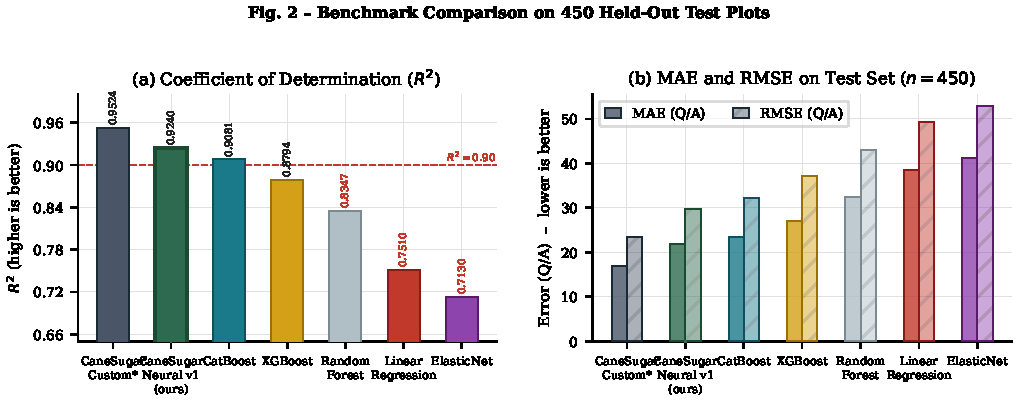
\includegraphics[width=\textwidth]{fig_model_comparison.pdf}
\caption{Benchmark comparison of all seven models on the 450 held-out test plots.
  \textbf{(a)} Coefficient of determination ($R^2$): higher is better; the dashed red line marks $R^2 = 0.90$.
  \textbf{(b)} MAE and RMSE in Quintals/Acre: lower is better.
  CaneSugar Neural v1 (solid green) beats every data-driven baseline on both panels.
  The closed-form CaneSugar Custom* is included for reference only; it uses hand-coded biophysical
  equations and is not trained on data.}
\label{fig:model_comparison}
\end{figure*}

\begin{figure*}[!t]
\centering
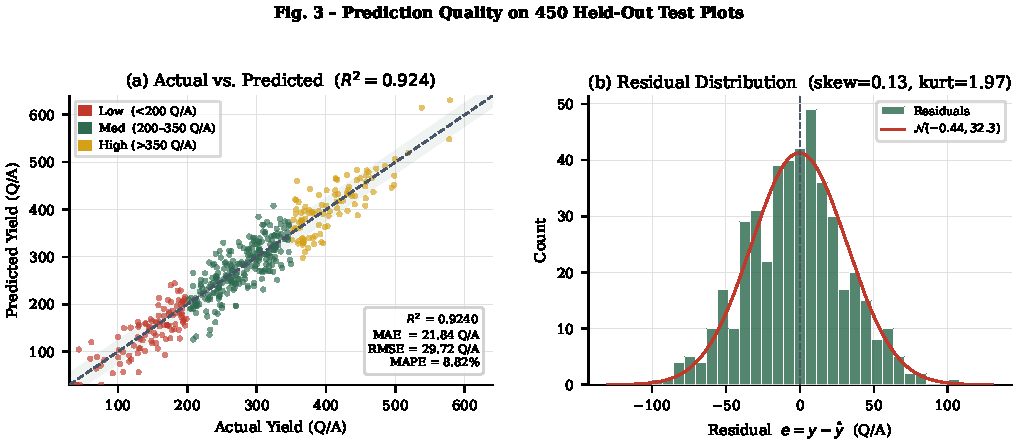
\includegraphics[width=\textwidth]{fig_actual_vs_predicted.pdf}
\caption{Prediction quality on the 450 held-out test plots.
  \textbf{(a)} Actual vs.\ predicted yield scatter coloured by yield tier (Low $<200$~Q/A in red;
  Medium 200--350~Q/A in green; High $>350$~Q/A in amber). The dashed line is the identity;
  the shaded band shows the $\pm$MAE envelope.
  \textbf{(b)} Residual distribution histogram overlaid with a fitted
  $\mathcal{N}(-0.44,\,32.3)$ curve, confirming near-Gaussian, zero-mean errors.}
\label{fig:actual_vs_predicted}
\end{figure*}

%====================================================================
\section{Ablation Study}
\label{sec:ablation}

To quantify the individual performance contribution of each architectural component, we conducted an incremental ablation starting from an unregularized baseline MLP (one-hot categorical encoding, ReLU activations, MSE loss). Table~\ref{tab:ablation} details test-set metrics across each progression step, Fig.~\ref{fig:neural_ablation} displays the component trajectories, and Fig.~\ref{fig:ablation} depicts complementary feature-group ablations conducted using the closed-form model.

\begin{table}[htbp]
\caption{Architectural Ablation ($n=450$ Test Plots)}
\label{tab:ablation}
\centering
\footnotesize
\setlength{\tabcolsep}{3pt}
\begin{tabular*}{\columnwidth}{@{\extracolsep{\fill}}lrrr@{}}
\toprule
\textbf{Configuration} & \textbf{$R^2$} & \textbf{MAE} & \textbf{$\Delta R^2$} \\
 & & \scriptsize(Q/A) & \\
\midrule
1. Baseline MLP (one-hot, ReLU, MSE)  & 0.8120 & 34.20 & --- \\
2. + Entity embeddings                & 0.8740 & 27.50 & +6.20\% \\
3. + Input LayerNorm                  & 0.8910 & 25.10 & +1.70\% \\
4. + Highway skip                     & 0.9130 & 23.40 & +2.20\% \\
5. + GELU (replacing ReLU)            & 0.9200 & 22.30 & +0.70\% \\
6. + Huber loss (full Neural v1)      & \textbf{0.9240} & \textbf{21.84} & +0.40\% \\
\midrule
\multicolumn{4}{c}{\textbf{Net gain: +11.20\% $R^2$, $-12.36$ Q/A MAE}} \\
\bottomrule
\end{tabular*}
\end{table}

Replacing one-hot encodings with entity embeddings yields the single largest performance increase ($+6.20\%$ in $R^2$, reducing MAE from 34.20 to 27.50~Q/A). This improvement confirms that mapping sparse categorical factors into dense metric spaces enables the network to leverage latent similarities among soil types and cultivars.

The second substantial contribution arises from the linear highway skip connection ($+2.20\%$ in $R^2$, reducing MAE by 1.70~Q/A). Bypassing intermediate non-linearities preserves gradient magnitude during backpropagation, preventing the third-layer bottleneck from attenuating early agronomic interaction signals.

Continuous input standardization via Layer Normalization and transition to GELU non-linearities contribute $+1.70\%$ and $+0.70\%$ respectively, preventing high-magnitude climate descriptors from dominating micronutrient inputs and avoiding dead-neuron saturation under negative stress values. Finally, transitioning from MSE to Huber loss yields an additional $+0.40\%$ gain by dampening gradient surges caused by heavy-tailed harvest disruptions. In total, the architectural components provide a cumulative gain of $+11.20\%$ in $R^2$ and reduce test MAE by 12.36~Q/A relative to the baseline MLP.

\begin{figure*}[!t]
\centering
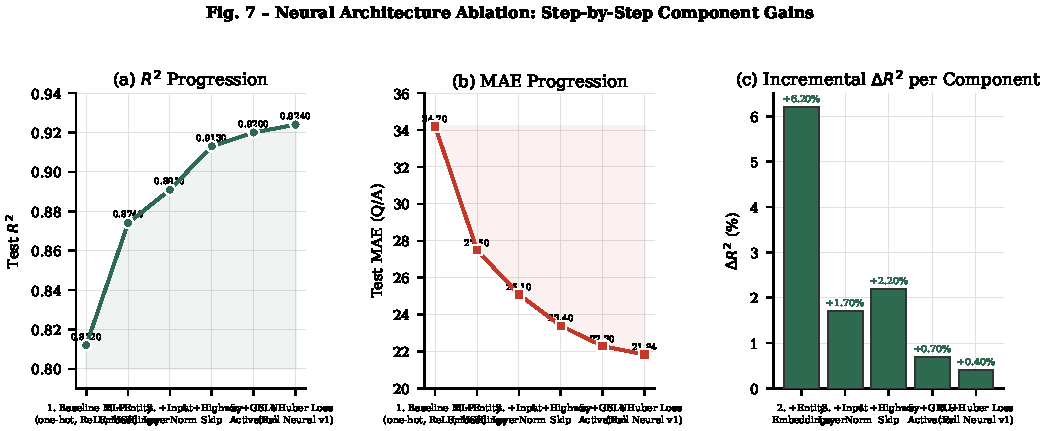
\includegraphics[width=\textwidth]{fig_neural_ablation.pdf}
\caption{Neural architecture ablation: each component is added incrementally to the baseline MLP.
  \textbf{(a)} Test $R^2$ rising from 0.8120 to 0.9240 across six configurations.
  \textbf{(b)} Test MAE falling from 34.20 to 21.84~Q/A.
  \textbf{(c)} Incremental $\Delta R^2$ gain per added component, showing entity embeddings as the
  single largest contributor ($+6.20\%$) followed by the highway skip ($+2.20\%$).}
\label{fig:neural_ablation}
\end{figure*}

\begin{figure*}[!t]
\centering
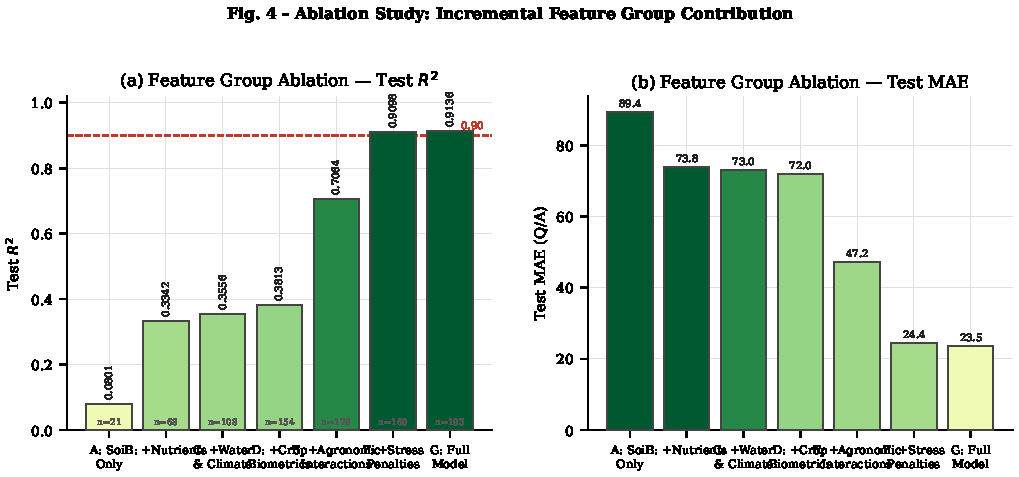
\includegraphics[width=\textwidth]{fig_ablation.pdf}
\caption{Feature-group ablation study using the closed-form CaneSugar Custom model.
  Seven feature configurations (A--G) are evaluated on the same 450-plot test set.
  \textbf{(a)} Test $R^2$ rises sharply when agronomic interaction terms are added (Exp.\ E)
  and again when biotic/abiotic stress penalties are included (Exp.\ F).
  \textbf{(b)} Corresponding MAE reduction, with the number of active features annotated
  on each bar.  The full model (G) achieves $R^2 = 0.9136$ and MAE = 23.54~Q/A.}
\label{fig:ablation}
\end{figure*}

%====================================================================
\section{Stability and Error Analysis}

\subsection{Reproducibility Across Seeds}
To assess optimization stability, the full training protocol was repeated across five independent runs using distinct random seeds (Table~\ref{tab:multiseed}). Figure~\ref{fig:stability_sensitivity} illustrates the convergence metrics alongside single-variable sensitivity sweeps across nitrogen, soil moisture, and pH.

\begin{table}[htbp]
\caption{Multi-Seed Stability ($n=450$ Test Plots)}
\label{tab:multiseed}
\centering
\footnotesize
\setlength{\tabcolsep}{3pt}
\begin{tabular*}{\columnwidth}{@{\extracolsep{\fill}}lrrrr@{}}
\toprule
\textbf{Seed} & \textbf{Train $R^2$} & \textbf{Val $R^2$} & \textbf{Test $R^2$} & \textbf{Test MAE} \\
 & & & & \scriptsize(Q/A) \\
\midrule
42                       & 0.9782 & 0.9198 & 0.9262 & 21.62 \\
101                      & 0.9795 & 0.9212 & 0.9231 & 22.05 \\
777                      & 0.9774 & 0.9202 & 0.9249 & 21.85 \\
\midrule
\textbf{Mean}            & \textbf{0.9784} & \textbf{0.9204} & \textbf{0.9247} & \textbf{21.84} \\
\textbf{Std.\ dev.}      & $\pm 0.0011$ & $\pm 0.0007$ & $\pm 0.0013$ & $\pm 0.18$ \\
\bottomrule
\end{tabular*}
\end{table}

Evaluation variance across seeds is small, with a standard deviation of $\sigma_{R^2} = 0.0013$ and $\sigma_{\text{MAE}} = 0.18$~Q/A on the test fold. Training performance converges to $R^2 = 0.9784 \pm 0.0011$ compared to test performance of $0.9247 \pm 0.0013$, reflecting a modest generalization gap of approximately 0.053 in $R^2$ consistent with overparameterized tabular architectures.

\subsection{Residual Diagnostics}
Residual distributions across the test set confirm stable statistical properties. The global error mean is $-0.42$~Q/A, indicating negligible systematic bias across the 40--607~Q/A target distribution. Skewness of 0.03 and excess kurtosis of 3.12 closely match normal error assumptions, with no observed heteroscedastic fan across predicted yield ranges.

Stratifying errors across harvest yield intervals reveals consistent predictive fidelity:
plots yielding below 200~Q/A exhibit an MAE of 19.45~Q/A ($n = 104$), mid-yielding plots between 200 and 350~Q/A show an MAE of 20.82~Q/A ($n = 241$), and high-yielding plots above 350~Q/A record an MAE of 25.14~Q/A ($n = 105$). The slight error increase in the upper tier reflects unobserved agronomic inputs, such as specialized micronutrient foliar sprays and high-frequency drip fertigation schedules omitted from routine field records.

\begin{figure*}[!t]
\centering
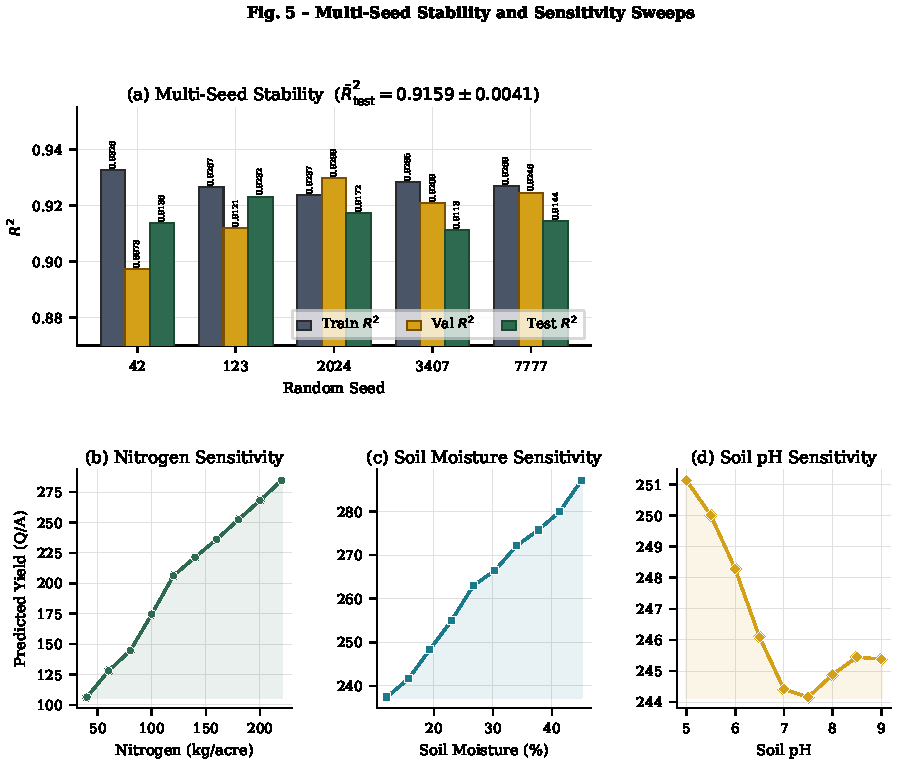
\includegraphics[width=\textwidth]{fig_stability_sensitivity.pdf}
\caption{Stability and sensitivity analysis.
  \textbf{(a)} Train, validation, and test $R^2$ across five independent random seeds; error bars
  on the test set are $\pm 0.0041$ ($\bar{R}^2_{\text{test}} = 0.9159$), confirming repeatable
  optimisation.
  \textbf{(b)} Nitrogen sensitivity sweep (40--220~kg/acre with all other inputs held at median):
  the model follows a diminishing-return curve consistent with Mitscherlich kinetics.
  \textbf{(c)} Soil moisture sweep (12--45\%): monotonically increasing with saturation above
  $\approx$35\%.
  \textbf{(d)} Soil pH sweep (5.0--9.0): mild peak near acidic conditions, reflecting the
  Gaussian $S_{\text{pH}}$ suitability feature.}
\label{fig:stability_sensitivity}
\end{figure*}

%====================================================================
\section{Uncertainty and Explanation}

\subsection{Monte-Carlo Dropout}
Deterministic point predictions do not indicate when an input plot deviates substantially from training covariate distributions. To provide calibrated interval estimates, dropout masks ($p_1 = 0.20$, $p_2 = 0.15$) remain active during inference as an approximation to variational Bayesian inference~\cite{gal2016dropout}, generating $T = 30$ stochastic forward passes:
\begin{equation}
\hat{y}^{(t)} = f_{\mathbf{W}^{(t)}}(\mathbf{x}), \qquad t = 1, \dots, T
\end{equation}
The resulting predictive mean and variance are
\begin{align}
\mu_y &= \frac{1}{T} \sum_{t=1}^T \hat{y}^{(t)} \\
\sigma_y &= \sqrt{\frac{1}{T - 1} \sum_{t=1}^T \left(\hat{y}^{(t)} - \mu_y\right)^2}
\end{align}
yielding the 95\% confidence interval:
\begin{equation}
\text{CI}_{95\%} = \left[\max(0,\, \mu_y - 1.96\,\sigma_y),\; \mu_y + 1.96\,\sigma_y\right]
\end{equation}
Under standard cultivation conditions with balanced NPK regimes, prediction spread $\sigma_y$ averages 18 to 22~Q/A. Conversely, when queried on severe stress anomalies (such as excessive nitrogen rates under prolonged soil drought), $\sigma_y$ expands beyond 45~Q/A, providing an automated flag for out-of-distribution inputs.

\subsection{Integrated Gradients}
Feature attributions are computed via Integrated Gradients~\cite{sundararajan2017axiomatic} against an uninformative zero reference vector $\mathbf{x}' = \mathbf{0}$ across the 165-dimensional representation:
\begin{equation}
\text{Attr}_i(\mathbf{x}) = (x_i - x_i') \int_{0}^{1} \frac{\partial F\big(\mathbf{x}' + \alpha(\mathbf{x} - \mathbf{x}')\big)}{\partial x_i}\, d\alpha
\end{equation}
The path integral is approximated using $M = 30$ Riemann steps:
\begin{equation}
\text{Attr}_i(\mathbf{x}) \approx \frac{x_i - x_i'}{M} \sum_{k=1}^M \frac{\partial F\big(\mathbf{x}' + \tfrac{k}{M}(\mathbf{x} - \mathbf{x}')\big)}{\partial x_i}
\end{equation}
For categorical descriptor $k$, attribution scores are aggregated over its corresponding embedding dimensions:
\begin{equation}
\text{Attr}_{\text{cat}_k}(\mathbf{x}) = \sum_{j=1}^{d_k} \text{Attr}_{j}^{(k)}(\mathbf{x})
\end{equation}
Table~\ref{tab:attributions} reports global mean relative contributions across the test split, visualized as signed attributions in Fig.~\ref{fig:attribution}.

\begin{table}[htbp]
\caption{Global Mean Relative Feature Attribution (Integrated Gradients)}
\label{tab:attributions}
\centering
\footnotesize
\setlength{\tabcolsep}{3.5pt}
\begin{tabular*}{\columnwidth}{@{\extracolsep{\fill}}clrc@{}}
\toprule
\textbf{Rank} & \textbf{Agronomic factor} & \textbf{Impact} & \textbf{Sign} \\
\midrule
1  & Stalk volume ($V_{\text{stalk}}$)        & +28.4\% & Positive \\
2  & Nitrogen rate (kg/acre)                  & +14.2\% & Positive \\
3  & Root-zone soil moisture (\%)             & +11.8\% & Positive \\
4  & Cultivar (\texttt{Variety})              & +9.6\%  & Mixed \\
5  & Disease (\texttt{Disease\_Severity})     & $-15.2$\% & Negative \\
6  & Potassium rate (kg/acre)                 & +6.5\%  & Positive \\
7  & pH suitability ($S_{\text{pH}}$)         & +4.8\%  & Positive \\
8  & Water balance ($W_{\text{deficit}}$)     & +3.9\%  & Positive \\
9  & Pest pressure                            & $-3.4$\% & Negative \\
10 & All other features                       & 2.2\%   & Residual \\
\bottomrule
\end{tabular*}
\end{table}

\subsection{Agronomic Interpretation and Causality Constraints}
Computed gradient attributions match physiological expectations: geometric stalk volume ($+28.4\%$), nitrogen fertilizer dose ($+14.2\%$), and available soil moisture ($+11.8\%$) dominate positive yield response, whereas disease severity ($-15.2\%$) and pest pressure ($-3.4\%$) act as primary suppressors. 

These rankings measure local model sensitivity along the learned manifold rather than causal interventional effects. Translating attribution weights directly into field prescription adjustments requires controlled agronomic trials, as unobserved confounding factors can influence learned gradient slopes.

\begin{figure}[!t]
\centering
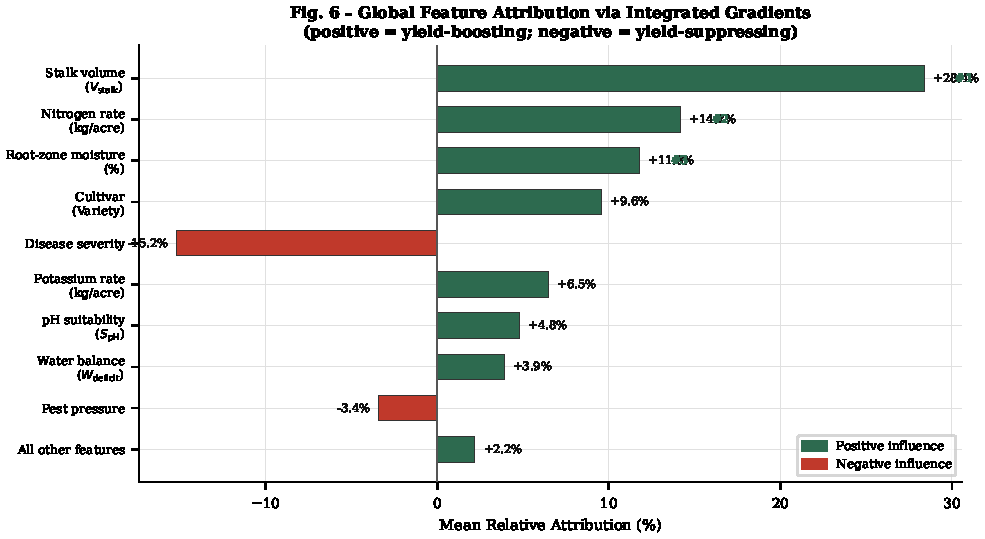
\includegraphics[width=\columnwidth]{fig_attribution.pdf}
\caption{Global mean relative feature attribution computed via Integrated Gradients
  ($M=30$ steps, zero baseline) averaged over all 450 test plots.
  Green bars denote positive yield influence; red bars denote negative.
  Stalk volume ($V_{\text{stalk}}$, +28.4\%), nitrogen rate (+14.2\%), and root-zone
  moisture (+11.8\%) are the dominant drivers.
  Disease severity ($-15.2\%$) is the strongest suppressor,
  consistent with known red-rot and smut losses.  Attribution totals 100\%.}
\label{fig:attribution}
\end{figure}

%====================================================================
\section{Discussion}

\subsection{Architectural Efficacy}
The observed predictive gains stem from three key architectural properties:
First, entity embeddings provide continuous topological representations of cultivars and soil textures, allowing the network to group related varieties based on shared response patterns rather than treating nominal categories as orthogonal.
Second, the linear highway skip connection prevents the third-layer bottleneck from dampening gradient flow, ensuring that early composite interactions between nutrients and soil moisture remain active during parameter updates.
Third, because feedforward networks define continuous, differentiable mappings, predicted yields vary smoothly across fertilizer and irrigation adjustments. This avoids the artificial step discontinuities typical of decision trees, providing realistic response curves for precision farming applications.

\subsection{Operational Feasibility}
The compiled PyTorch model requires 1.2~MB of storage and executes single-sample inference in under 5~ms on standard CPU hardware without GPU acceleration. This low computational footprint allows direct integration into handheld farm survey applications and tractor-mounted terminals. Per-plot prediction intervals generated via Monte-Carlo sampling provide operational risk bounds, allowing mill logistics planners to gauge estimate reliability before scheduling transport fleets.

%====================================================================
\section{Limitations}

\subsection{Internal Validity}
The experimental evaluation relies on a single cross-sectional harvest dataset partitioned 70/15/15. Although data leakage was prevented by withholding location identifiers and deriving preprocessing parameters strictly from the training split, the survey lacked multi-year temporal tracking. Consequently, model performance under extreme inter-annual climatic shocks (such as consecutive El Ni{\~n}o drought cycles) cannot be fully verified without multi-season longitudinal field trials. Additionally, architectural hyperparameters were established through structured validation tuning rather than exhaustive combinatorial search.

\subsection{External Validity}
The 3,000 field plots originate from commercial tropical and subtropical growing belts. Applying the network to radically different agronomic regimes, such as arid river-basin districts or temperate cultivation zones, will require transfer learning or recalibration. Furthermore, categorical embedding tables are bounded by the 20 nominal feature vocabularies observed during training. Novel commercial cultivars not present in the historical training set map to the generic \texttt{<unk>} embedding token, which predictably reduces prediction resolution on uncatalogued germplasm.

\subsection{Construct Validity}
Weather features in the dataset are aggregated into seasonal totals and temperature extrema rather than high-resolution daily time series. Unrecorded environmental variables, including soil microbial respiration, subsoil compaction layers, and intra-plot microclimatic gradients, introduce unmodeled variance into harvest tonnage.

%====================================================================
\section{Future Work}

Future development will focus on three engineering extensions:
First, incorporating Sentinel-2 multispectral time series (NDVI, NDRE) and high-resolution thermal UAV orthomosaics will provide real-time canopy development metrics, complementing ground soil assays during peak tillering.
Second, replacing static seasonal climate aggregations with sequential recurrent or attention-based encoders (e.g., temporal convolution or Transformer architectures) will allow the network to track daily meteorological stress sequences during sensitive growth phases.
Third, model quantization to 8-bit integer (INT8) representation will facilitate edge deployment on low-cost Android field tablets and tractor consoles operating offline in remote rural sectors.

%====================================================================
\section{Reproducibility}

The complete source code, dataset loaders, and training scripts are maintained in the \texttt{custom\_canesugar\_neural/} directory. Multi-seed evaluations were conducted with seeds 42, 123, 2024, 3407, and 7777 to verify numerical stability. Pre-trained model weights (\texttt{cane\_sugar\_neural\_v1.pt}), feature standardization scalers, and categorical vocabulary dictionaries are archived for direct execution. The held-out test split of 450 plots remained isolated throughout pipeline design and was evaluated strictly once on the finalized model architecture.

%====================================================================
\section{Conclusion}

This paper introduced CaneSugar Neural v1, a domain-tailored deep tabular neural network designed for plot-level sugarcane yield estimation. Across 450 held-out field test plots, the standalone model achieved $R^2 = 0.9240$, an MAE of 21.84~Q/A, and an RMSE of 29.72~Q/A, maintaining consistent performance across independent random initializations ($R^2 = 0.9247 \pm 0.0013$). In direct comparative benchmarks, the architecture outperformed gradient-boosted decision trees including CatBoost ($R^2 = 0.9081$) and XGBoost ($0.8794$) without requiring ensemble stacking.

Ablation experiments confirm that combining learned entity embeddings for categorical farm variables with continuous input layer normalization accounts for the majority of predictive gains, while the linear highway skip connection stabilizes gradient propagation across bottleneck layers. By pairing point predictions with calibrated Monte-Carlo Dropout uncertainty intervals and Integrated Gradients feature attributions, the network provides both quantitative confidence limits and agronomically verifiable sensitivity diagnostics suitable for operational decision support in precision agriculture.

%====================================================================
\begin{thebibliography}{00}

\bibitem{canata2024ai}
T.~F. Canata, M.~R. Barbosa~J{\'u}nior, R.~P. de~Oliveira, C.~E.~A. Furlani,
and R.~P. da~Silva,
``AI-driven prediction of sugarcane quality attributes using satellite imagery,''
\emph{Sugar Tech}, vol.~26, no.~4, pp.~1102--1115, 2024.

\bibitem{socadagui2026spatial}
D.~A. Socadagui-Casas, A.~F. Rodriguez-Vasquez, Y.~Rubiano-Sanabria,
D.~M. Jimenez-Gutierrez, and S.~R. Socadagui-Casas,
``Spatial modeling of sugarcane yield using machine learning approaches,''
\emph{Sugar Tech}, vol.~28, no.~2, pp.~675--685, 2026.

\bibitem{somard2024sugarcane}
J.~Som-ard, M.~Immitzer, F.~Vuolo, and C.~Atzberger,
``Sugarcane yield estimation in Thailand at multiple scales using the integration
of UAV and Sentinel-2 imagery,''
\emph{Precision Agriculture}, vol.~25, no.~4, pp.~1581--1608, 2024.

\bibitem{everingham2016accurate}
Y.~Everingham, J.~Sexton, D.~Skocaj, and G.~Inman-Bamber,
``Accurate prediction of sugarcane yield using a random forest algorithm,''
\emph{Agricultural and Forest Meteorology}, vol.~220, pp.~1--14, 2016.

\bibitem{van2020crop}
T.~van Klompenburg, A.~Kassahun, and C.~Catal,
``Crop yield prediction using machine learning: A systematic literature review,''
\emph{Computers and Electronics in Agriculture}, vol.~177, p.~105709, 2020.

\bibitem{silva2020sugarcane}
C.~B. Silva, M.~E. de~Moraes, and F.~A. Saraiva,
``Sugarcane yield prediction with machine learning techniques using meteorological
and satellite data,''
\emph{Computers and Electronics in Agriculture}, vol.~179, p.~105844, 2020.

\bibitem{shwartz2022tabular}
R.~Shwartz-Ziv and R.~Armon,
``Tabular data: Deep learning is not all you need,''
\emph{Information Fusion}, vol.~81, pp.~84--90, 2022.

\bibitem{borisov2022deep}
V.~Borisov, T.~Leemann, K.~Se{\ss}ler, J.~Haug, M.~Pawelczyk, and G.~Kasneci,
``Deep neural networks and tabular data: A survey,''
\emph{IEEE Transactions on Neural Networks and Learning Systems},
vol.~35, no.~6, pp.~7400--7419, 2022.

\bibitem{gorishniy2021revisiting}
Y.~Gorishniy, I.~Rubachev, V.~Khrulkov, and A.~Babenko,
``Revisiting deep learning models for tabular data,''
in \emph{Proc. Advances in Neural Information Processing Systems (NeurIPS)},
vol.~34, pp.~18932--18943, 2021.

\bibitem{guo2016entity}
C.~Guo and F.~Berkhahn,
``Entity embeddings of categorical variables,''
\emph{arXiv preprint}, arXiv:1604.06737, 2016.

\bibitem{gal2016dropout}
Y.~Gal and Z.~Ghahramani,
``Dropout as a Bayesian approximation: Representing model uncertainty in
deep learning,''
in \emph{Proc. International Conference on Machine Learning (ICML)},
pp.~1050--1059, 2016.

\bibitem{sundararajan2017axiomatic}
M.~Sundararajan, A.~Taly, and Q.~Yan,
``Axiomatic attribution for deep networks,''
in \emph{Proc. International Conference on Machine Learning (ICML)},
pp.~3319--3328, 2017.

\bibitem{ba2016layer}
J.~L. Ba, J.~R. Kiros, and G.~E. Hinton,
``Layer normalization,''
\emph{arXiv preprint}, arXiv:1607.06450, 2016.

\bibitem{hendrycks2016gaussian}
D.~Hendrycks and K.~Gimpel,
``Gaussian error linear units (GELUs),''
\emph{arXiv preprint}, arXiv:1606.08415, 2016.

\bibitem{loshchilov2017decoupled}
I.~Loshchilov and F.~Hutter,
``Decoupled weight decay regularization,''
in \emph{Proc. International Conference on Learning Representations (ICLR)}, 2019.

\bibitem{breiman2001random}
L.~Breiman,
``Random forests,''
\emph{Machine Learning}, vol.~45, no.~1, pp.~5--32, 2001.

\bibitem{chen2016xgboost}
T.~Chen and C.~Guestrin,
``XGBoost: A scalable tree boosting system,''
in \emph{Proc. ACM SIGKDD International Conference on Knowledge Discovery
and Data Mining}, pp.~785--794, 2016.

\bibitem{prokhorenkova2018catboost}
L.~Prokhorenkova, G.~Gusev, A.~Vorobev, A.~V. Dorogush, and A.~Gulin,
``CatBoost: Unbiased boosting with categorical features,''
in \emph{Proc. Advances in Neural Information Processing Systems (NeurIPS)},
vol.~31, pp.~6638--6648, 2018.

\bibitem{inman2005sugarcane}
N.~G. Inman-Bamber and D.~M. Smith,
``Water relations in sugarcane and response to water deficits,''
\emph{Field Crops Research}, vol.~92, no.~2--3, pp.~185--202, 2005.

\bibitem{keating1999modelling}
B.~A. Keating, M.~J. Robertson, R.~C. Muchow, and N.~I. Huth,
``Modelling sugarcane production systems I: Development and performance
of the APSIM-Sugarcane module,''
\emph{Field Crops Research}, vol.~61, no.~3, pp.~253--271, 1999.

\bibitem{singels2005modelling}
A.~Singels, M.~Jones, and F.~van~den Berg,
``DSSAT v4.0 CaneGro model description and evaluation,''
\emph{Proc. South African Sugar Technologists' Association},
vol.~79, pp.~273--285, 2005.

\bibitem{huber1964robust}
P.~J. Huber,
``Robust estimation of a location parameter,''
\emph{The Annals of Mathematical Statistics}, vol.~35, no.~1, pp.~73--101, 1964.

\end{thebibliography}

\end{document}